\section{Test particles}\label{sec:testparticles}

Decoupling matter sources from Einstein's equations tests whether trajectory updates, metric reconstruction, source deposition, and interior excision remain accurate before self-gravity acts. In this test-particle regime, macroparticles follow timelike geodesics of a prescribed or independently evolved vacuum geometry while deposited moments $(E, S_i, S_{ij})$ remain passive diagnostics. Holding back-reaction off permits direct comparison with exact geodesics and published benchmarks \cite{Wu:2026nrpic} in units of the black hole ADM mass $M$.

\subsection{Fixed black hole}\label{sec:fixed_black_hole}

Integrating bound orbits around a spinning black hole tests whether the pushers preserve relativistic integrability and precession over many dynamical periods. In Boyer--Lindquist or spherical Kerr--Schild coordinates $(t, r, \theta, \phi)$ around a Kerr black hole of spin $a$, timelike geodesics conserve the Killing energy $\Egeo$, axial angular momentum $L_z$, and Carter constant $Q$ \cite{1985ApJ...298...34S},
\begin{align}\label{eq:kerr_invariants}
\Egeo &= -u_t, \qquad L_z = u_\phi, \nonumber\\
Q &= u_\theta^2 + \cos^2\theta\left[a^2\bigl(1 - \Egeo^2\bigr) + \frac{L_z^2}{\sin^2\theta}\right].
\end{align}
In the nonrotating limit ($a \to 0$), spherical symmetry reduces $Q$ to $L^2 - L_z^2$ for total angular momentum $L$. For spin $a = 0.9\,M$, equatorial eccentric and inclined Boyer--Lindquist orbits stay on their invariant tori over many radial periods (Fig.~\ref{fig:orbits}). Both pushers match exact apsidal and nodal precession with bounded invariant errors and convergent fixed-point iterations. Because the Boyer--Lindquist spatial metric is diagonal, both tetrad gauges coincide there, while the midpoint update conserves cyclic $L_z$ to rounding error \cite{Bacchini:2020cze}.

\begin{figure*}[t]
\centering
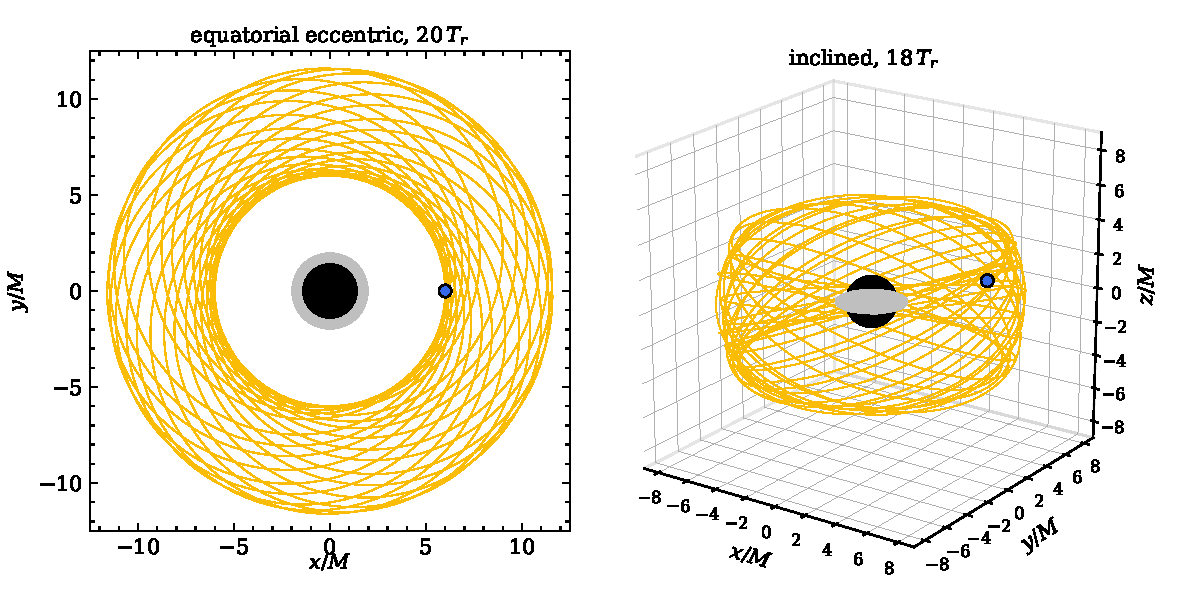
\includegraphics[width=\textwidth]{figures/fig_bl_trajectories.pdf}
\caption{Bound test-particle trajectories around a Kerr black hole ($a = 0.9\,M$) precess coherently and stay confined to their invariant tori. Left: equatorial eccentric orbit; right: inclined three-dimensional orbit [check]. Solid yellow curves show the spacetime Boris pusher in the symmetric gauge on the analytic Boyer--Lindquist metric from initial blue markers outside the black event horizon and gray ergosphere [check].}
\label{fig:orbits}
\end{figure*}

Sending a particle onto a near-capture eccentric trajectory tests whether the implicit midpoint pusher reproduces the strong-field invariant accuracy in Ref.~\cite{Wu:2026nrpic}. In Kerr--Schild coordinates, an inclined passage ($a = 0.9\,M$, $e = 0.99$) grazes the event horizon before returning outward (Fig.~\ref{fig:passage}). Because the midpoint update of Sec.~\ref{sec:pushers} depends solely on the coordinate metric and its spatial derivatives, its discrete trajectory is uniquely fixed. On the analytic spherical Kerr--Schild metric, the implicit midpoint pusher conserves cyclic $L_z$ to rounding error and reproduces all published digits of the maximum relative errors in $\Egeo$ and $Q$ \cite{Wu:2026nrpic}. On the Cartesian Kerr--Schild metric reconstructed via the Hermite weights of Sec.~\ref{sec:reconstruction}, where the grid breaks continuous axisymmetry, it again matches all published digits for $\Egeo$, $L_z$, and $Q$ \cite{Wu:2026nrpic}.

\begin{figure*}[t]
\centering
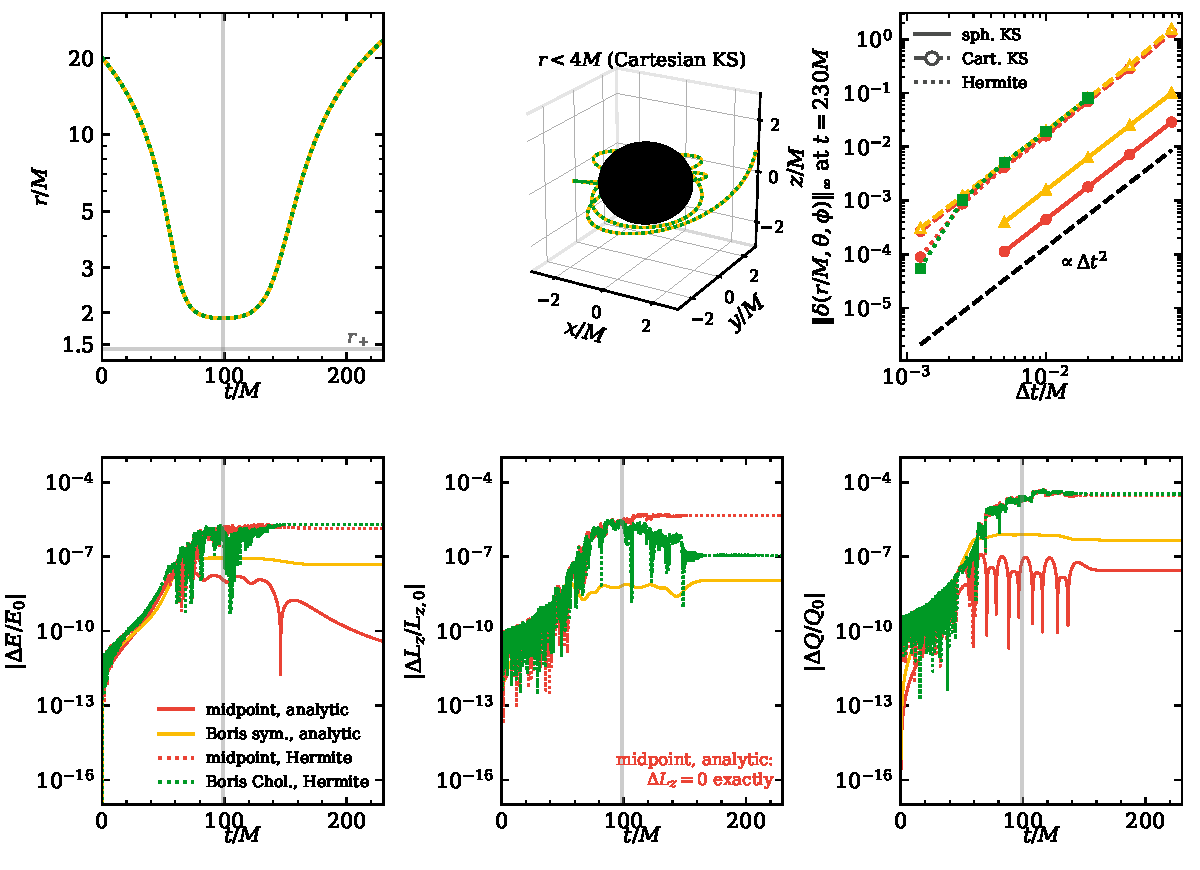
\includegraphics[width=\textwidth]{figures/fig_ks_passage.pdf}
\caption{Both pushers conserve $(\Egeo, L_z, Q)$ through a near-capture Kerr passage ($a = 0.9\,M$, $e = 0.99$), with mesh reconstruction setting the invariant floor and trajectories converging as $\Delta t^2$. Top: radius, near-horizon trajectory, and position error versus $\Delta t$ with a $\Delta t^2$ guide (black dashed); bottom: invariant errors across periapsis (gray) [check]. Colors mark exact or published references (blue), the implicit midpoint pusher (red), and the spacetime Boris pusher in the symmetric (yellow) and Cholesky (green) gauges [check]. Line styles mark analytic spherical (solid), analytic Cartesian (dashed), and mesh-reconstructed (dotted) metrics [check].}
\label{fig:passage}
\end{figure*}

Applying the spacetime Boris pusher to the same passage determines which local orthonormal frames reproduce the published analytic and mesh benchmarks. Off-diagonal spatial metric components in Kerr--Schild coordinates distinguish the symmetric gauge from the Cholesky gauge. Continuous geodesics are frame independent because triad connections in the tetrad equation of motion cancel endpoint projections identically. Over a finite step $\Delta t$, midpoint evaluation of the Boris rotation of Sec.~\ref{sec:pushers} leaves a gauge-dependent second-order error. Reference~\cite{Wu:2026nrpic} leaves the tetrad gauge unspecified. For analytic spherical Kerr--Schild input, the symmetric gauge reproduces all published digits of the $\Egeo$, $L_z$, and $Q$ errors in Ref.~\cite{Wu:2026nrpic} (Fig.~\ref{fig:passage}), while the $(r, \theta, \phi)$ Cholesky gauge gives distinct errors. For mesh-reconstructed Cartesian input, the $(x, y, z)$ Cholesky gauge reproduces all published digits, while the symmetric gauge and permuted Cholesky orderings give distinct values.

Varying the time step $\Delta t$ and cell spacing $h$ independently establishes how trajectory and invariant errors converge across spinning and nonrotating black hole spacetimes. On analytic metrics, position and invariant errors of both pushers and gauges converge at second order in $\Delta t$ across the Kerr orbits and $e = 0.99$ passage (Fig.~\ref{fig:passage}). In the nonrotating limit ($a \to 0$), circular, inclined eccentric, and plunging orbits are tested against exact Schwarzschild solutions (Fig.~\ref{fig:convergence}). Spherical Kerr--Schild circular motion advances linearly in time and azimuth and integrates to rounding error. Cartesian Kerr--Schild circular, eccentric, and horizon-crossing plunging orbits all converge as $\Delta t^2$. Multi-block Cartesian mesh runs at small $\Delta t$ match virtual-lattice runs of spacing $h$ to rounding error across block interfaces. Refining $h$ reduces metric, position, and invariant errors at the third-order rate of cubic Hermite reconstruction for $a = 0.9\,M$ and $a \to 0$ (Fig.~\ref{fig:convergence}).

\begin{figure*}[t]
\centering
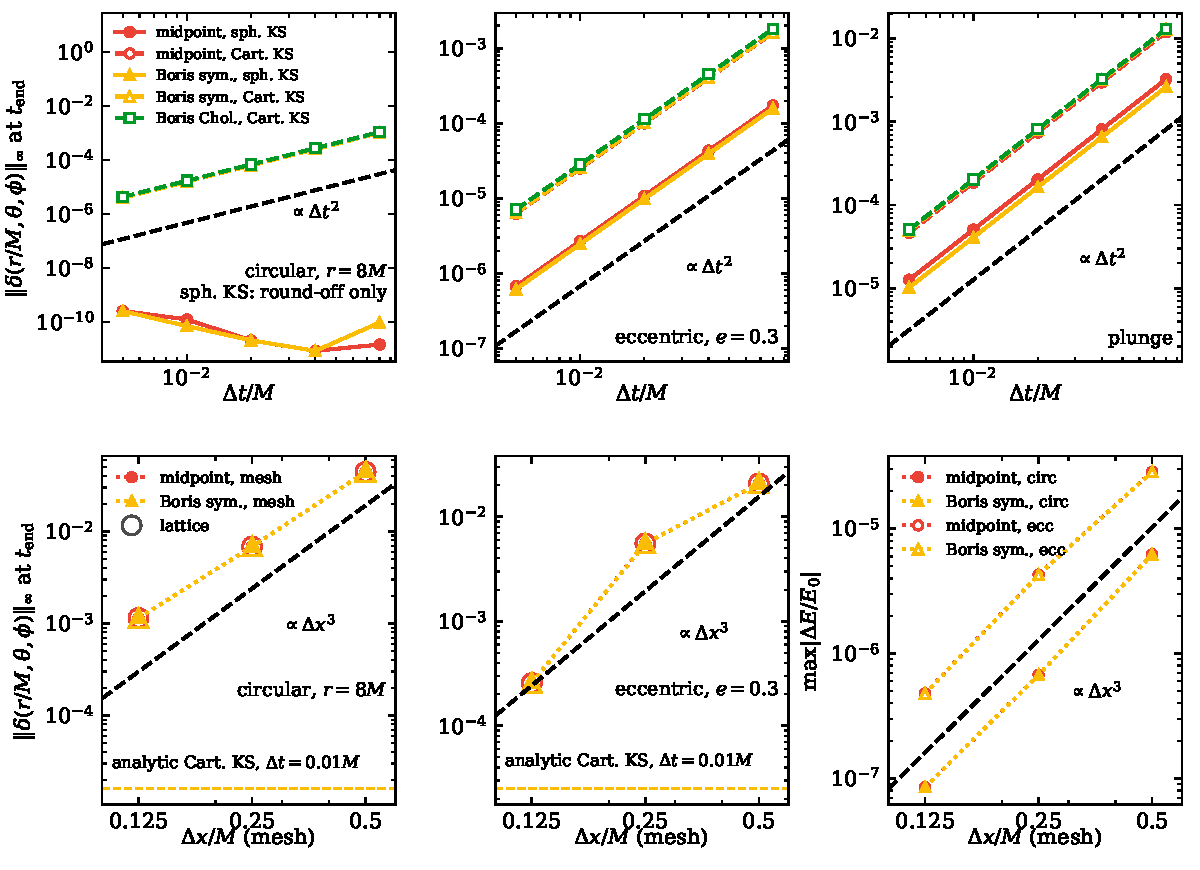
\includegraphics[width=\textwidth]{figures/fig_schwarzschild_convergence.pdf}
\caption{In the nonrotating limit ($a \to 0$), trajectories converge at second order in $\Delta t$ on analytic metrics and at third order in cell spacing $h$ under cubic Hermite reconstruction. Top: position error versus $\Delta t$ for circular, eccentric, and plunging orbits; bottom: position and $\Egeo$ errors versus $h$ on the mesh (dotted) and virtual lattice (open markers) with power-law guides (black dashed) [check]. Curves show the implicit midpoint pusher (red) and the spacetime Boris pusher in the symmetric (yellow) and Cholesky (green) gauges on analytic spherical (solid) and Cartesian (dashed) metrics [check].}
\label{fig:convergence}
\end{figure*}

Comparing mesh-reconstructed trajectories against exact analytic Cartesian trajectories settles whether spatial interpolation or time-stepping truncation governs the Cartesian position error on the $e = 0.99$ passage. Reference~\cite{Wu:2026nrpic} attributes the grid error of both pushers on this passage to spacetime interpolation. Sweeping $\Delta t$ on the analytic Cartesian Kerr--Schild metric alongside the Hermite grid at fixed $h$ separates both effects (Fig.~\ref{fig:passage}). Spatial interpolation dominates the $(\Egeo, L_z, Q)$ errors, which exceed analytic Cartesian values at the published step size and flatten onto an interpolation floor as $\Delta t$ shrinks. Conversely, the analytic Cartesian run without interpolation gives nearly the same final-position error at the published step size as the Hermite grid, and both fall as $\Delta t^2$. Differencing grid and analytic-Cartesian final states at equal $\Delta t$ confirms that pure interpolation shifts the position far less than Cartesian time-stepping until the finest $\Delta t$ tested.

Replacing a single orbit with a cloud of macroparticles tests whether phase mixing on a refined mesh preserves single-particle invariants and analytic trajectories. Gaussian clouds of $N = 10^2$, $10^3$, and $10^4$ bound test particles are initialized around an equatorial circular orbit for $a = 0.9\,M$ and $a \to 0$. Each cloud evolves on both the analytic Cartesian metric and a statically refined octree mesh with passive deposition. Differential orbital shear stretches each cloud into an arc, a trailing spiral, and an azimuthally mixed ring tracked by the deposited energy density $E$ \cite{2008gady.book.....B} (Fig.~\ref{fig:tpcluster}). Vertical epicycles and Kerr nodal precession set the ring thickness. Every macroparticle keeps bounded $(\Egeo, L_z, Q)$ errors free of secular drift, independently of $N$. On the mesh, both pushers give indistinguishable third-order-convergent invariant errors set by Hermite reconstruction and closely match the analytic positions and mixing histories.

\begin{figure*}[t]
\centering
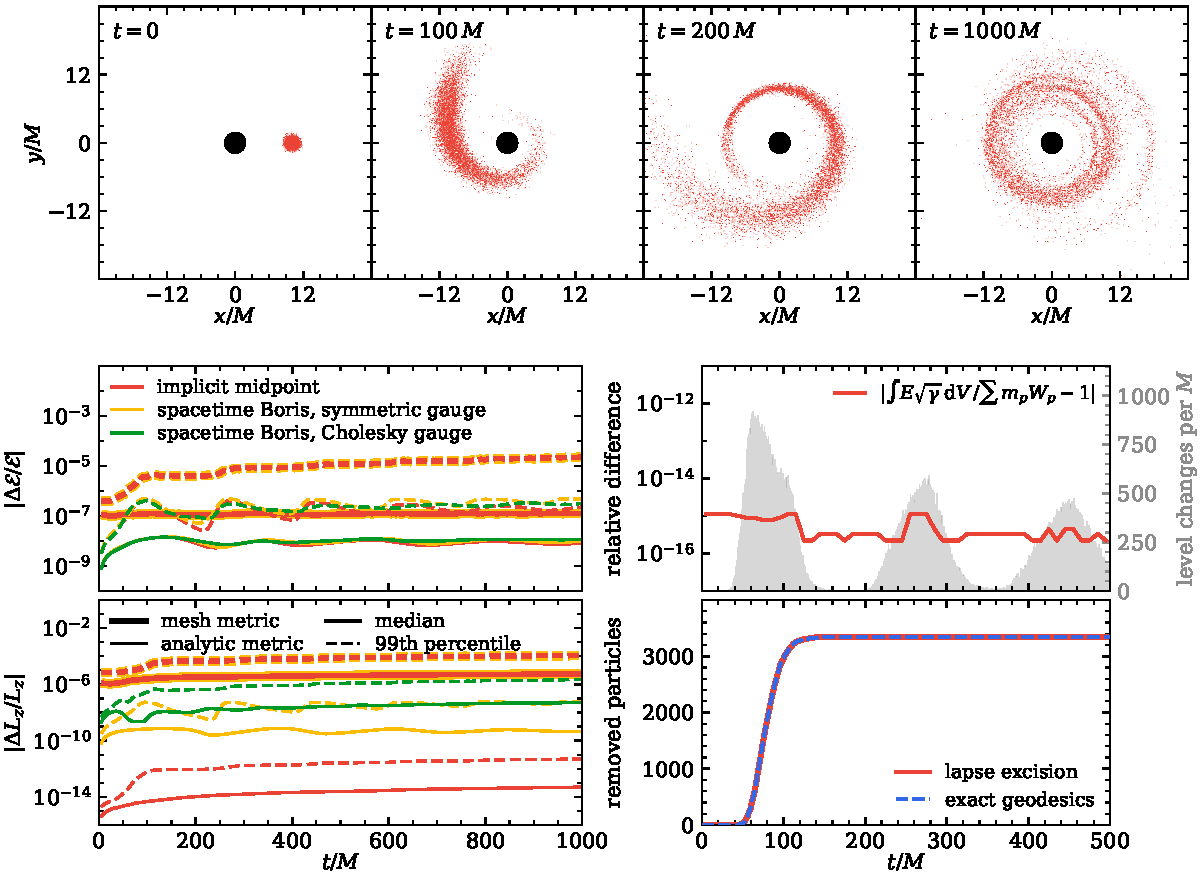
\includegraphics[width=\textwidth]{figures/fig_tp_cluster.pdf}
\caption{A test-particle cluster ($N = 10^4$) around a Kerr black hole ($a = 0.9\,M$) phase-mixes into a ring while conserving single-particle invariants, preserving pre-filter source integrals, and matching exact lapse-excision counts. Panels show phase-mixing snapshots, invariant errors, pre- and post-filter residuals of the conservation identity, and cumulative excised counts [check]. Curves show exact references (blue), the implicit midpoint pusher (red), and the spacetime Boris pusher in the symmetric (yellow) and Cholesky (green) gauges on analytic (solid) and mesh-reconstructed (dotted) metrics [check].}
\label{fig:tpcluster}
\end{figure*}

Accumulating stress-energy from thousands of orbiting macroparticles tests how multi-level deposition and mesh filtering conserve total energy and momentum across refinement boundaries. During phase mixing and infall, macroparticles cross static octree interfaces repeatedly while depositing $(E, S_i, S_{ij})$ in the uncapped limit of the level cap of Sec.~\ref{sec:deposition}. Before filtering, the conservation identity holds to rounding error across all level crossings and excisions whenever clouds lie at least half a cell inside the outer boundary (Fig.~\ref{fig:tpcluster}). For the few large-apocenter particles within half a cell of the outer boundary, cloud weight outside the domain accounts to rounding error for the difference. Subsequent binomial filtering on leaf cells breaks exact conservation at a small level, a limitation of mesh-level smoothing. Averaging $(E, S_i, S_{ij})$ across spatially varying $\sqrt{\gamma}$ and coarse-fine ghost zones shifts proper-volume integrals by a small fraction per boundary-crossing particle (Fig.~\ref{fig:tpcluster}).

Lowering the cluster angular momentum across the capture threshold and varying $N$ test whether lapse excision matches exact geodesic predictions and how sampling noise scales. Plunging-family clusters ($N = 10^4$) for $a = 0.9\,M$ and $a \to 0$ send a large fraction of macroparticles across the event horizon, with exact Kerr effective potentials predicting arrival times at $\aexc$. With both pushers on the mesh, lapse excision matches the predicted removal curve up to a few marginal near-separatrix orbits perturbed across the barrier by interpolation (Fig.~\ref{fig:tpcluster}). Active, excised, and escaped rest masses sum to the initial cluster mass to rounding error. Across independent bound clusters of $N = 10^2$, $10^3$, and $10^4$ macroparticles at fixed total mass, pairwise root-mean-square differences in filtered $E$ fall as $N^{-1/2}$ while diffuse rings remain sampling-noise dominated.

\subsection{Evolving black hole}\label{sec:evolving_black_hole}

Evolving the black hole spacetime dynamically in moving-puncture gauge raises the question of how physical geodesic accuracy can be separated from coordinate drift. A nonrotating vacuum black hole puncture of initial mass $M$ evolves on a statically refined Cartesian mesh under Z4c in moving-puncture gauge (Sec.~\ref{sec:spacetime}) from time-symmetric data with precollapsed lapse. Zero-mass tracers advance on the time-averaged Hermite-reconstructed metric via the implicit midpoint pusher. As $1+\log$ slicing and the Gamma-driver shift relax the slice toward a stationary trumpet \cite{Campanelli:2005dd,Baker:2005vv,Hannam:2008sg}, coordinates drift outward and the coordinate energy $\alpha W - \beta^i u_i$ swings during the gauge transient. Comparison with exact Schwarzschild geodesics therefore uses gauge-independent worldline observables: orbital azimuth, the areal radius $R$ of the sphere of proper area $4\pi R^2$ passing through the particle, and proper time
\begin{equation}\label{eq:particle_proper_time}
\tau(t) = \int_0^t \frac{\alpha}{W}\,\dd t'.
\end{equation}

Tracking radially infalling and plunging tracers tests whether worldlines follow exact strong-field geodesics through the evolving horizon to interior excision. A radial infaller from rest and an inspiraling plunger cross refinement boundaries smoothly, pass the apparent horizon, and undergo lapse excision at $\aexc$ (Fig.~\ref{fig:tracers}). Along radial infall, $R(\tau)$ tracks the exact Schwarzschild cycloid closely outside the horizon, deviating only within a few cells of the puncture where steep gradients limit interpolation of $R$. Along the slower plunge, $R(\tau)$ and azimuth accumulate a small advance relative to the exact geodesic of initial mass $M$. Reintegrating the exact geodesic from the post-transient state with the evolved slice Misner--Sharp mass removes nearly that entire offset (Fig.~\ref{fig:tracers}).

\begin{figure*}[t]
\centering
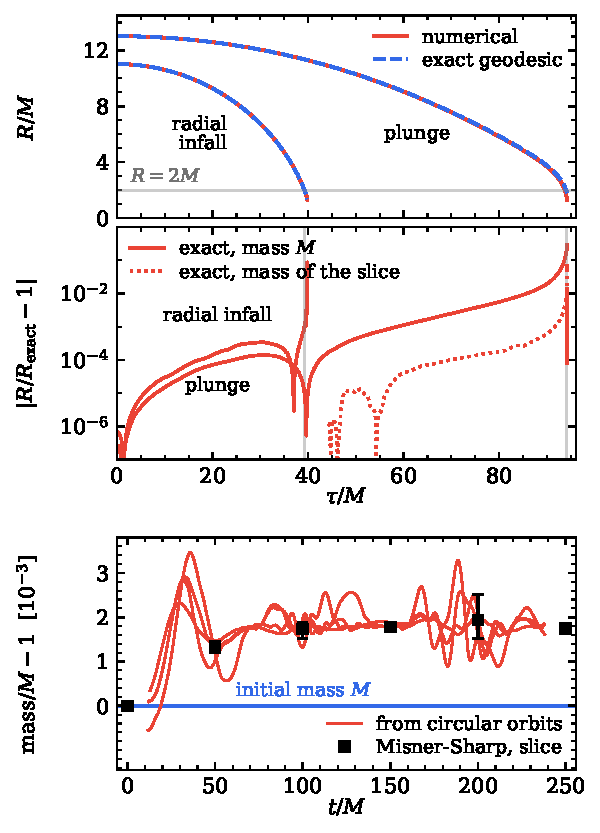
\includegraphics[width=\textwidth]{figures/fig_tracers.pdf}
\caption{Test particles on a numerically evolved moving-puncture black hole spacetime track exact geodesics of the evolved slice in gauge-independent observables. Panels show areal radius $R$ versus proper time $\tau$ with residuals for radial infall and plunge, plus the enclosed mass implied by circular tracers versus slice Misner--Sharp mass [check]. Curves compare exact Schwarzschild geodesics of the initial and evolved masses (blue) with implicit midpoint pusher trajectories on the reconstructed mesh metric (red dotted) [check].}
\label{fig:tracers}
\end{figure*}

Following circular tracers over many dynamical times determines whether their small radial offset reflects pusher error or the evolved black hole slice mass. Equatorial and inclined circular tracers keep planar orbits and conserved angular momentum $L$ while their coordinate radii drift outward and their areal radii $R$ oscillate slightly inside their initial values. Saved spatial slices show that after the early evolution at this resolution, the exterior settles into a uniform Schwarzschild slice whose Misner--Sharp mass is slightly heavier than $M$. Carrying the angular momentum of mass $M$, each tracer starts at the apocenter of a mildly eccentric orbit of that heavier black hole, whose geodesics reproduce the $R(\tau)$ oscillations. In Schwarzschild geometry, areal radius $R$, angular momentum $L$, and radial acceleration imply an enclosed mass
\begin{equation}\label{eq:implied_mass}
M_{\rm eff} = \frac{L^2/R - R^2\,\dd^2 R/\dd\tau^2}{1 + 3L^2/R^2}.
\end{equation}
Across all orbital radii and inclinations, $M_{\rm eff}$ agrees with the slice Misner--Sharp mass (Fig.~\ref{fig:tracers}). Extending these gauge-independent tracer tests to an inspiraling and merging binary black hole in moving-puncture gauge is in progress [pending].
